\chapter{Problema 2}

\section{Descripción del problema}

Una empresa realiza planificaciones de viajes aéreos entre \textit{n} ciudades. Para ir de una ciudad \textit{i} a una ciudad \textit{j} puede ser necesario coger varios vuelos distintos. El tiempo de un vuelo directo de \textit{i} a \textit{j} será (si existe) \textit{T(i,j)} (que puede ser distinto de \textit{T(j,i}). Hay que tener en cuenta que si cogemos un vuelo de \textit{i} a \textit{k} y después otro de \textit{k} a \textit{j}, será necesario esperar un tiempo de \textit{escala} adicional \textit{E(k)} en el aeropuerto de \textit{k}, con lo que el tiempo de ese viaje de \textit{i} a \textit{j} será de \textit{T(i,k) + T(k,j) + E(k)}.

Se desea conocer la forma de volar desde cualquier ciudad \textit{i} hasta cualquier otra \textit{j} en el menor tiempo posible. Diseñad e implementad un algoritmo de Programación dinámica que resuelva este problema. Aplicadlo para resolver el problema, para n=4, cuya matriz de tiempos es la siguiente, suponiendo que \textit{E(k)} = 1 para cualquier valor de k.

\begin{figure}
    \centering
    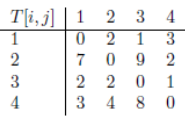
\includegraphics[width=0.5\linewidth]{figures/problema2/tabla2.png}
\end{figure}

\section{Solución: Diseño de componentes y del algoritmo}


\subsection{Resolución del problema por etapas}

La forma de resolver cada etapa será elegir si tardamos menos tiempo tomando un vuelo directo al destino final o haciendo escala en otro aeropuerto y luego tomar un vuelo al destino final. En esta comparación habrá que tener en cuenta la posibilidad de hacer escala en cualquiera de los 2 aeropuertos restantes que tenemos, ya que no tendrá sentido hacer escala en el aeropuerto del que salimos o al que pretendemos llegar ya que realmente no estaríamos haciendo escala alguna, tan solo sumaríamos el coste de estar haciendo una escala que no existe. 

Realmente lo que usaremos será el Algoritmo de Floyd (con alguna pequeña modificación para que sea más entendible), pues el problema se puede ver como calcular el camino más corto que une un par de vértices de un grafo.

\subsection{Ecuación recurrente}

La ecuación recurrente constará, por tanto, de calcular el mínimo de entre tomar un vuelo directo o hacer escala en un aeropuerto distinto tanto al de origen como el de llegada y luego ir al destino final.
\[
tiempo\_minimo(i, j) =  \min \begin{cases} 
tiempo (i, j) \\
tiempo\_min(i, k) + tiempo\_min(k, j) + E(k) para todo k!=i,j\\
\end{cases}
\]

El caso base del que partimos es la matriz de tiempos inicial, es decir, \(tiempo\_min_{0}(i,j) = tiempo(i,j)\)

Realmente es hacer un mínimo entre 3 cosas, el coste de ir directo y el coste de hacer escala en los otros 2 aeropuertos restantes que no sean ni el punto de partida ni el punto de llegada, ya que entonces no estaríamos haciendo escala alguna, más el coste de hacer escala y luego hacer otro vuelo al destino final.

\subsection{Valor objetivo}

Se desea conocer el valor \textit{tiempo\_minimo(i,j)}, el tiempo mínimo que se puede tardar en ir de un aeropuerto \textit{i} a otro aeropuerto \textit{j} dados una serie de duraciones de vuelos entre diversos aeropuertos y el coste \textit{E(k)} de hacer escalas.

\subsection{Verificación del cumplimiento del P.O.B}

El principio de optimalidad de Bellman se verifica cuando toda solución óptima está compuesta por soluciones óptimas de sus subproblemas. En nuestro caso, las soluciones óptimas de los subproblemas se obtienen al calcular el tiempo mínimo que se tarda en ir entre cada par de nodos (al calcularse como el mínimo de todas las posibilidades para ir a ese punto ya sea de forma directa o haciendo escala, podemos considerar que esa solución será óptima). De esta forma, cuando tengamos que construir una solución óptima final para un origen y destino concretos, lo estaremos haciendo a partir de soluciones óptimas de los subproblemas ya calculados. Al asegurar que los viajes más cortos encontrados entre todos los aeropuertos son compuestos de subviajes que también son las más cortos posibles, podemos concluir que se cumple el principio de optimalidad de Bellman.

\subsection{Diseño de la memoria}

Para el diseño de la memoria, decidimos usar una matriz en la que almacenar los tiempos mínimos ya calculados para ir de un aeropuerto \textit{i} a otro aeropuerto \textit{j}. Para futuras ejecuciones del algoritmo, antes de usarlo bastará con comprobar si el valor en la casilla es válido (distinto de -1) o no para ver si es necesario ejecutar el algoritmo o simplemente basta con recuperar el valor deseado porque se haya calculado previamente.

Para ello, usamos una matriz en la que se irán almacenando los valores de tiempos mínimos calculados, la cual comenzará inicializada como la matriz de tiempos originales y sobre la cual se aplicará el Algoritmo de Floyd para hallar el camino más corto que une un par de vértices de un grafo, es decir, dos aeropuertos.

También iremos rellenando una matriz de antecesores, la cual nos será útil para realizar la recuperación de la solución, por lo que será explicado más tarde.

\subsection{Diseño del algoritmo de cálculo de coste óptimo}

Como ya hemos explicado anteriormente, tras aplicar el algoritmo de Floyd bastará con consultar la posición indicada de la matriz para saber cuál es el tiempo mínimo que se puede tardar en ir de un aeropuerto a otro, siendo el coste óptimo el mínimo entre tomar un vuelo directo y hacer escala en otros aeropuertos.

Con este diseño, construimos el algoritmo de Programación Dinámica como sigue:

\begin{lstlisting}
origen y destino -> aeropuertos de origen y destino
tiempos -> matriz de tiempos de vuelo directos entre aeropuertos
tiempos_min -> matriz de tiempos mínimos calculados
antecesores -> matriz donde almacenamos de qué aeropuerto venimos en cada iteracion del bucle. Inicialmente tendra el origen de los vuelos directos ya que no se consideran escalas.

tiempo_min (origen, destino, tiempos[nxn], tiempos_min[nxn], antecesores[nxn]){

    tiempos_min = tiempos
    Para cada k hasta n
        Para cada i hasta n
            Para cada j hasta n
                si k!=i,j // si realmente podemos hacer una escala
                    tiempos_min (i,j) = min (tiempos_min(i,j), tiempos_min(i,k) + tiempos_min(k,j) + 1)
                    si tiempos_min (i,j) == tiempos_min(i,j), tiempos_min(i,k) + tiempos_min(k,j) + 1 // si he hecho escala, modifico la matriz de antecesores para saber dónde he hecho escala
                        antecesores(i,j) = k
                    
    devolver tiempos_min(origen, destino)                   
}

\end{lstlisting}

\subsection{Diseño del algoritmo de recuperación de la solución}

Para recuperar la solución y ver en qué aeropuertos hemos hecho escala, bastará con ir rellenando una matriz de antecesores al mismo tiempo que calculamos las distancias mínimas. De esta forma, tras haber ejecutado el algoritmo bastará con ir consultando la tabla de adyacencia e ir consultando los valores de la misma hasta dar con una posición en el que ya se haya llegado al origen del viaje.

Inicialmente la tabla de antecesores almacenará el valor del aeropuerto desde el cual se hace el vuelo directo, ya que los tiempos mínimos comenzarán siendo los que se tardan en ir con vuelos directos y aún no se han considerado las escalas.

Al calcular los tiempos mínimos, si se ha hecho una escala se modifica la matriz de antecesores y se pone como valor el aeropuerto en el que se hace escala para poder llegar hasta el destino final. De esta forma, para recuperar el conjunto de aeropuertos que hay que recorrer para ir de un origen a un destino tendremos que ir moviéndonos por la matriz de antecesores comenzando por la casilla final a la que queremos ir hasta que lleguemos al punto en el que el antecesor sera el origen del que partimos. Iremos almacenando en el camino los aeropuertos que vamos visitando, aunque los almacenaremos en orden inverso y luego le tendremos que dar la vuelta para obtener la ruta realizada.

Con este diseño, construimos el algoritmo de recuperación de la solución como sigue:

\begin{lstlisting}
sol -> conjunto de aeropuertos visitados

recuperar_sol(origen, destino, antecesores[nxn]{
    sol = conjunto vacio
    sol = sol U {antecesores(origen, destino)} // Incluimos el aeropuerto final
    col = destino
    
    hacer{
        anterior = antecesores (origen,col)
        sol = sol U {anterior} // Aniadimos de donde venimos
        col = anterior // Para ver como hemos llegado hasta ahi la siguiente iteración
    } mientras que anterior != origen

    // Dar la vuelta a sol para tener ordenados los aeropuertos que visitamos

    devolver sol
}
\end{lstlisting}


